\section{Auswertung}
\subsection{Messung des Kontrasts}
Zur Bestimmung des Kontrastes des Interferometers wird ein Laser mit einer Wellenlänge von $\lambda = \SI{623,99}{\nano \meter}$ verwendet. Aus den in Tabelle \ref{tab:Kontrast} zu sehenden Werten wird der Kontrast 
\begin{equation}
    K_\text{exp} = \frac{U_\text{Max}-U_\text{Min}}{U_\text{Max}+U_\text{Min}}
\end{equation} 
berechnet.
\begin{table}[H] 
   \centering 
   \caption{Aufgenommene Messwerte zur Messung des Kontrastes.} 
   \label{tab:Kontrast} 
   \begin{tabular} { c c c c } 
 \toprule 
 {$Winkel\:/\: \mathrm{°}$} & {$U_\text{max}\:/\: \mathrm{mV}$} & {$U_\text{min}\:/\: \mathrm{mV}$} & {Kontrast}\\ 
    \midrule 
      0 & 1,12 & 0,90 & 0.1089108 \\ 
     15 & 2,10 & 0,73 & 0.4840989 \\ 
     30 & 2,90 & 0,33 & 0.7956656 \\ 
     45 & 3,45 & 0,15 & 0.9166666 \\ 
     60 & 2,94 & 0,25 & 0.8432601 \\ 
     75 & 1,98 & 0,69 & 0.4831460 \\ 
     90 & 1,16 & 0,98 & 0.0841121 \\ 
    105 & 1,25 & 0,39 & 0.5243902 \\ 
    120 & 1,02 & 0,08 & 0.8545454 \\ 
    135 & 0,89 & 0,03 & 0.9347826 \\ 
    150 & 0,82 & 0,20 & 0.6078431 \\ 
    165 & 0,88 & 0,38 & 0.3968254 \\ 
    180 & 1,03 & 0,86 & 0.0899470 \\ 
    \bottomrule 
  \end{tabular}
\end{table}


Die daraus erhaltenen Daten werden dann, wie in Abbildung \ref{fig:Kontrast} zu sehen ist, an die Funktion
\begin{equation}
    K = A \cdot | \sin{(2 \cdot \phi -\delta)} |
\end{equation}
\begin{center}
    \tiny{($A, \delta \hat{=} \text{Fitparameter} $)}
\end{center}
gefittet. 
\begin{figure}[H]
    \centering
    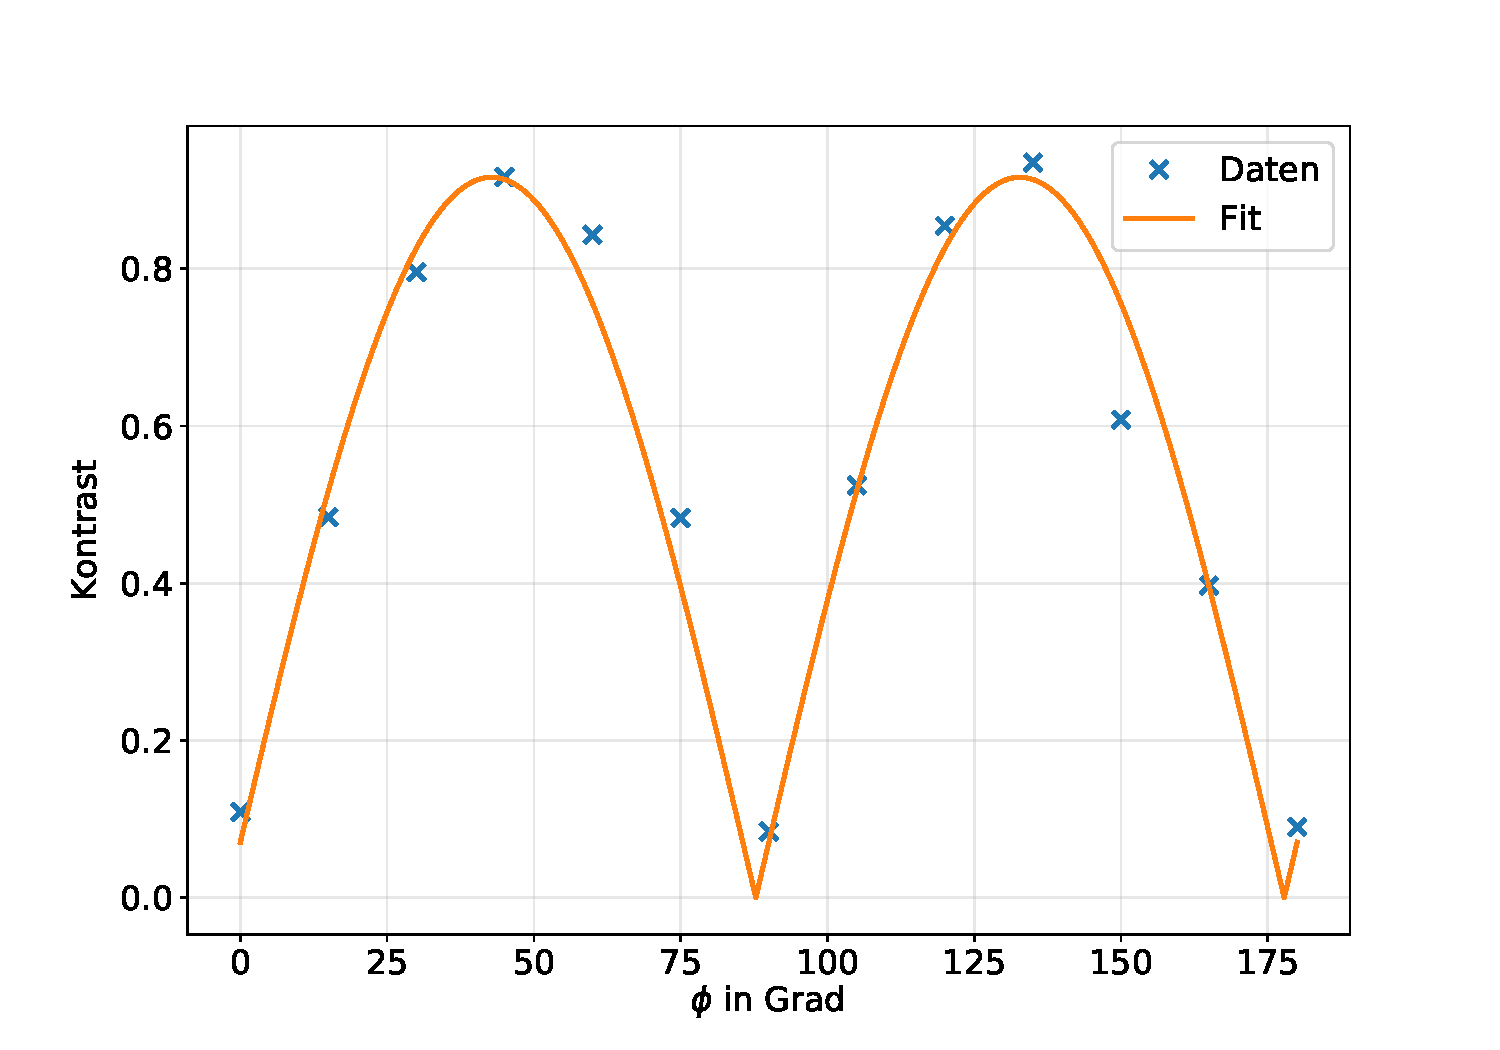
\includegraphics[width=0.8\textwidth]{data/kontrast.pdf}
    \caption{Messwerte für den winkelabhängigen Verlauf des Kontrastes.}
    \label{fig:Kontrast}
\end{figure}
Es ergeben sich die folgenden Fit-Parameter:
\begin{align}
       A &=  -0,077 \pm 0.026 \\
  \delta &=  0,916 \pm 0.025
\end{align}

\subsection{Bestimmung des Brechungsindex von Luft}
Der Brechungsindex für Luft ergibt sich aus dem Zusammenhang
\begin{equation}
    n = \frac{N \cdot \lambda}{L} + 1 .
\end{equation}
\begin{center}
    \tiny{($L \hat{=} \text{Länge der Gaszelle} = 10 \si{\centi \meter} $, $ N \hat{=} \text{Anzahl der Nulldurchgänge} $)} \label{eqn:n}
\end{center}
